\documentclass[10pt]{scrartcl}
\usepackage[english]{babel}
\usepackage{multirow}
\usepackage[default]{opensans}
\usepackage{sfmath} % sans font also for math
\usepackage[binary-units = true]{siunitx}
\usepackage{graphicx}
% defining the paper layout that no text overlaps with the header
\usepackage[
  top=35mm,
  headheight=25mm,
  headsep=3mm,
  bottom=30mm,
  left=25mm,
  right=25mm
]{geometry}

\usepackage[verbose]{placeins}
\usepackage{subcaption}
\usepackage{latexsym}
\usepackage[centertags]{amsmath}
\usepackage{amssymb}
\usepackage[]{glossaries}

\graphicspath{{figures/}}
% custom header and footpage
\usepackage{scrpage2}
\pagestyle{scrheadings} % you have to set the custom layout
% Head
%\chead{}
\ohead{
\includegraphics[height=25mm]{figures/EUCALL.png}}
% Foot
\ifoot{
\includegraphics[height=13.4mm]{figures/EU.png}} % left foot
\cfoot{%
  \begin{minipage}{100mm}%
    \begin{scriptsize}%
      \normalfont{This project has received funding from the}
      \textit{European Union’s Horizon 2020 research and innovation programme}
      \normalfont{under grant agreement No 654220.}
    \end{scriptsize}%
  \end{minipage}%
} % center foot
\ofoot{\thepage} % right foot

\usepackage{booktabs}

%%%%%%%%%%%%%%%%%%%%%%%%%%%%%%%%%%%%%%%%%%%%%%%
%   BIBLIOGRAPHY SETTINGS
\usepackage[bibstyle=nature,sorting=none,maxnames=1000,eprint=false,
defernumbers=true, backend=biber]{biblatex}
\usepackage{chemformula}
\usepackage{hyperref}


\renewcommand*\finalnamedelim{, and\addspace}
\DeclareNameAlias{sortname}{last-first}
\renewcommand{\newunitpunct}{, }

\AtEveryBibitem{%
  \clearfield{day}%
  \clearfield{month}%
  \clearfield{endday}%
  \clearfield{endmonth}%
  \clearfield{issn}%
  \clearfield{issue}%
}
%convert titles to hyperlinks using doi
\ExecuteBibliographyOptions{doi=true} \newbibmacro{string+doi}[1]{%
  \iffieldundef{doi}{#1}{\href{http://dx.doi.org/\thefield{doi}}{#1}}}
  \DeclareFieldFormat*{title}{\usebibmacro{string+doi}{\mkbibemph{#1}}}

\addbibresource{urls.bib}
\addbibresource{footnotes.bib}
\addbibresource{library.bib}

%%%%%%%%%%%%%%%%%%%%%%%%%%%%%%%%%%%%%%%%%%%%%%%
% GLOSSARY SETTINGS
\setacronymstyle{long-short}
\input{glossary}
\makeglossaries
%%%%%%%%%%%%%%%%%%%%%%%%%%%%%%%%%%%%%%%%%%%%%%%

% Zeilenabstand
\renewcommand{\baselinestretch}{1.2}



% sophisticated linking of references in the pdf and setting some options
\usepackage{url}                                                  % for correct typesettings of URLs
\usepackage{hyperref}                                             % for sophisticated linking of urls, dois, pictures, tables, etc.
\hypersetup{
    unicode=true,                                                 % non-Latin characters in Acrobat’s bookmarks
    pdftoolbar=true,                                              % show Acrobat’s toolbar?
    pdfmenubar=true,                                              % show Acrobat’s menu?
    pdffitwindow=false,                                           % window fit to page when opened
    pdfstartview={FitH},                                          % fits the width of the page to the window
    pdftitle={D4.4: Interoperable simulations},                                        % title
    pdfauthor={C. Fortmann-Grote},                                           % author
    pdfsubject={EUCALL WP4 (SIMEX) Deliverable D4.4},                             % subject of the document
    pdfcreator={pdflatex},                                         % creator of the document
    pdfkeywords={EUCALL, SIMEX, simulations, Rad-Hydro, XFEL, ESRF, warm dense
    matter, absorption, radiography},                                         % list of keywords
    pdfnewwindow=true,                                            % links in new PDF window
    colorlinks=true,                                              % false: boxed links; true: colored links
    linkcolor=blue,                                                % color of internal links (change box color with linkbordercolor)
    citecolor=blue,                                                % color of links to bibliography
    filecolor=blue,                                               % color of file links
    urlcolor=blue                                                 % color of external links
}

% Zeilenabstand
\renewcommand{\baselinestretch}{1.2}

\begin{document}
\makeatletter
\begin{titlepage}
\thispagestyle{scrheadings}
\begin{center}
$~$\\
\vspace{0cm}
{\Large\textbf{EUCALL}\\[2ex]
The European Cluster of Advanced Laser Light Sources}\\[4ex]
%
{\small\textbf{Grant Agreement number: 654220}}\\[8ex]
%
Work Package 4 -- SIMEX\\[4ex]
%
Deliverable D4.4\\
%
Simulated coherent scattering data from plasma and non--plasma samples\\[5ex]
%
Lead Beneficiary: European XFEL, HZDR\\[5ex]
%
Carsten Fortmann-Grote, Michael Bussmann,
  Marco Garten, Axel Huebl, Thomas Kluge,
  and Adrian P. Mancuso\\[4ex]
%
Due data: September 30, 2017\\
Delivery data: \today \\[4ex]
%
Project webpage: \url{www.eucall.eu}\\[6ex]
%
{%
\small
\begin{tabular}{|l|l|}
  \hline
  \multicolumn{2}{|l|}{ \textit{Deliverable Type} } \\
  \hline
  R = Report\hfill & R, OTHER \\
  DEM = Demonstrator, pilot, prototype, plan designs & \\
  DEC = Websites, patents filing, press \& media actions, videos, etc. & \\
  OTHER = Software, technical diagram, etc. & \\
  \hline
  \multicolumn{2}{|l|}{\textit{Dissemination level}} \\
  \hline
  PU = Public, fully open, e.g. web & PU \\
  CO = Confidential, restricted under conditions set out in Model Grant
  Agreement\hspace*{17ex}\  & \\
  CI = Classified, information as referred to in Commission Decision 2001/844/EC
  & \\
  \hline
\end{tabular}
}

\end{center}
%
%\vfill
\centering{%
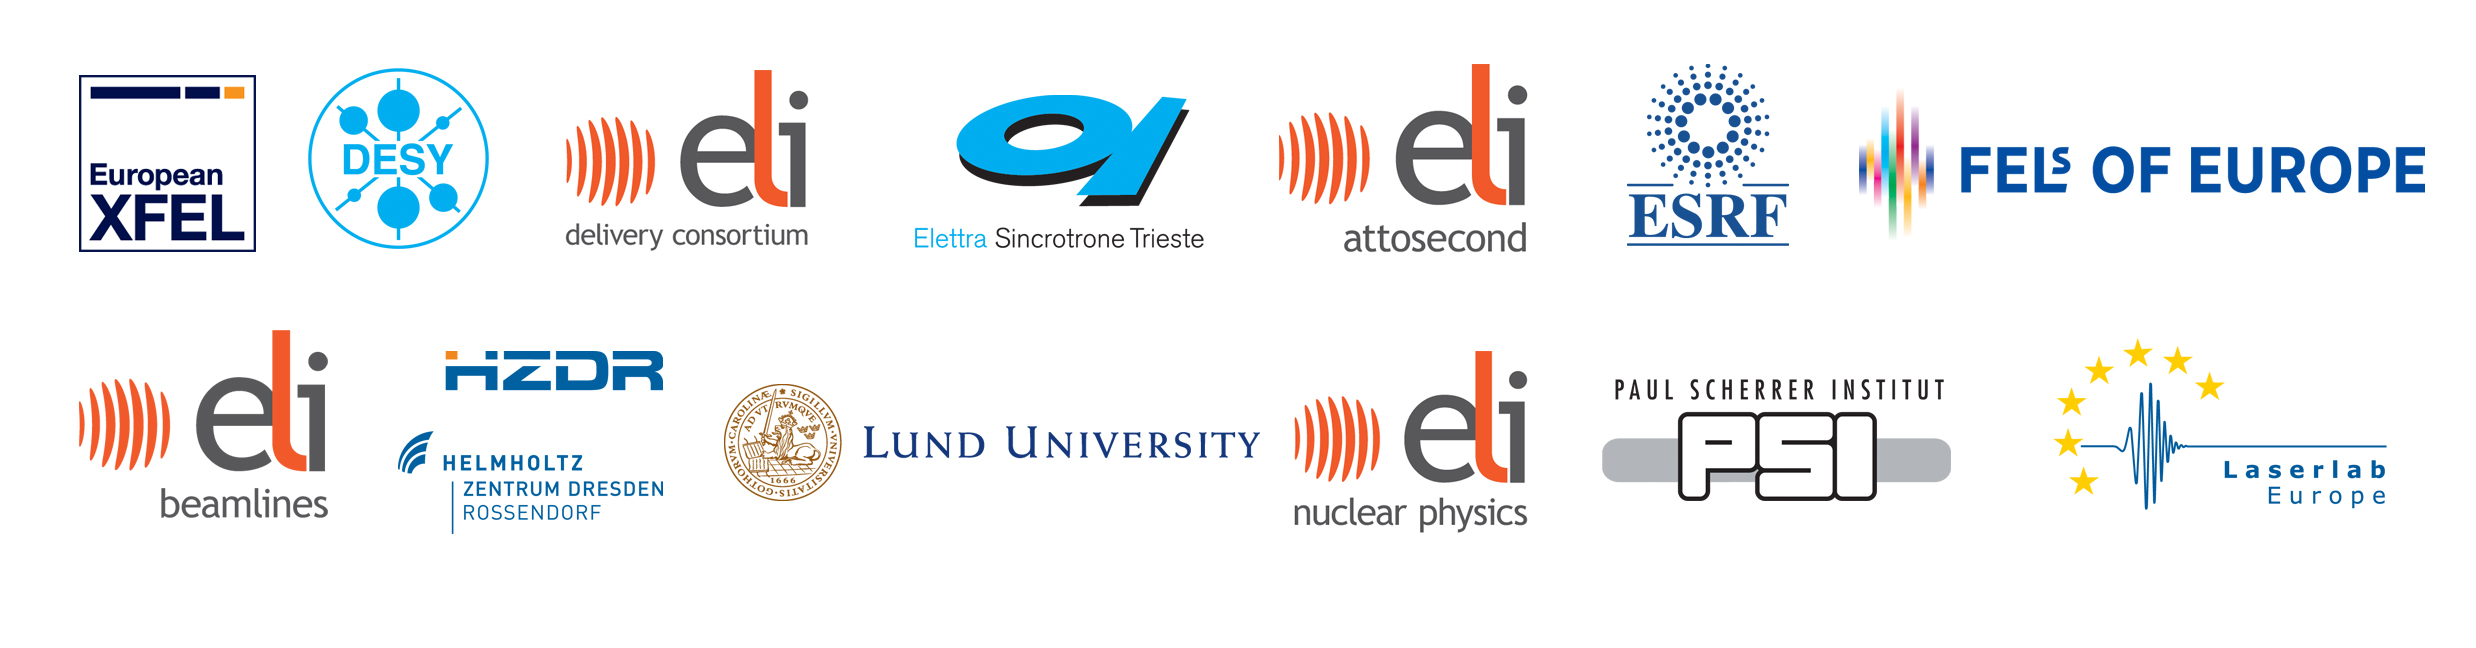
\includegraphics[width=0.91\textwidth]{figures/PartnerLogos_2017}
}
\normalfont
\end{titlepage}
\makeatother

%\tableofcontents

\section{Summary}
%
As first applications of our simulation software suite \textit{simex\_platform}
\cite{simex_github, Fortmann-Grote2017a, EUCALL_SIMEX_D4.3}, we have employed the simulation capabilities of
\textit{simex\_platform} \cite{simex_github} to simulate two photon experiments:
\begin{enumerate}
  \item Coherent diffraction from high--power laser excited optically thin and
    thick plasmas (plasma sample)
  \item Single particle imaging at the European XFEL (non--plasma sample)
\end{enumerate}

\section{Plasma sample}

In Deliverable Report D4.3~\cite{EUCALL_SIMEX_D4.3}, we present the interoperability of \gls{xfel} and \gls{uhi} laser pulse generation,
interaction with the target, and generation of a \gls{saxs} image using the
scattering code \textit{ParaTAXIS}.

A \gls{pic} simulation provides the time
evolution of the electron density on which the \gls{xfel} photons are scattered. We
assume invariance of the target in propagation direction and simulate the \gls{xfel}
pulse with \num{e12} photons for which the target is optically thin,
see left part of Fig. \ref{fig:scattering}. We further demonstrate
scattering on an optically thick setup by simulating
resonant scattering on the ions of the target. The ion density follows the
electron density as expected for plasma expansion into vacuum\cite{Mora2003},
see right part of Fig. \ref{fig:scattering}.

The signal of the optically thick target is washed out due to
higher scattering probability. In both, the optically thin and the optically
thick case, the
\gls{saxs} pattern well resolves the nanometer--scale grating depth and period, taking
into account the target evolution during the interaction time with the laser
pulse.
%
\begin{figure}[ht]
  \centering
  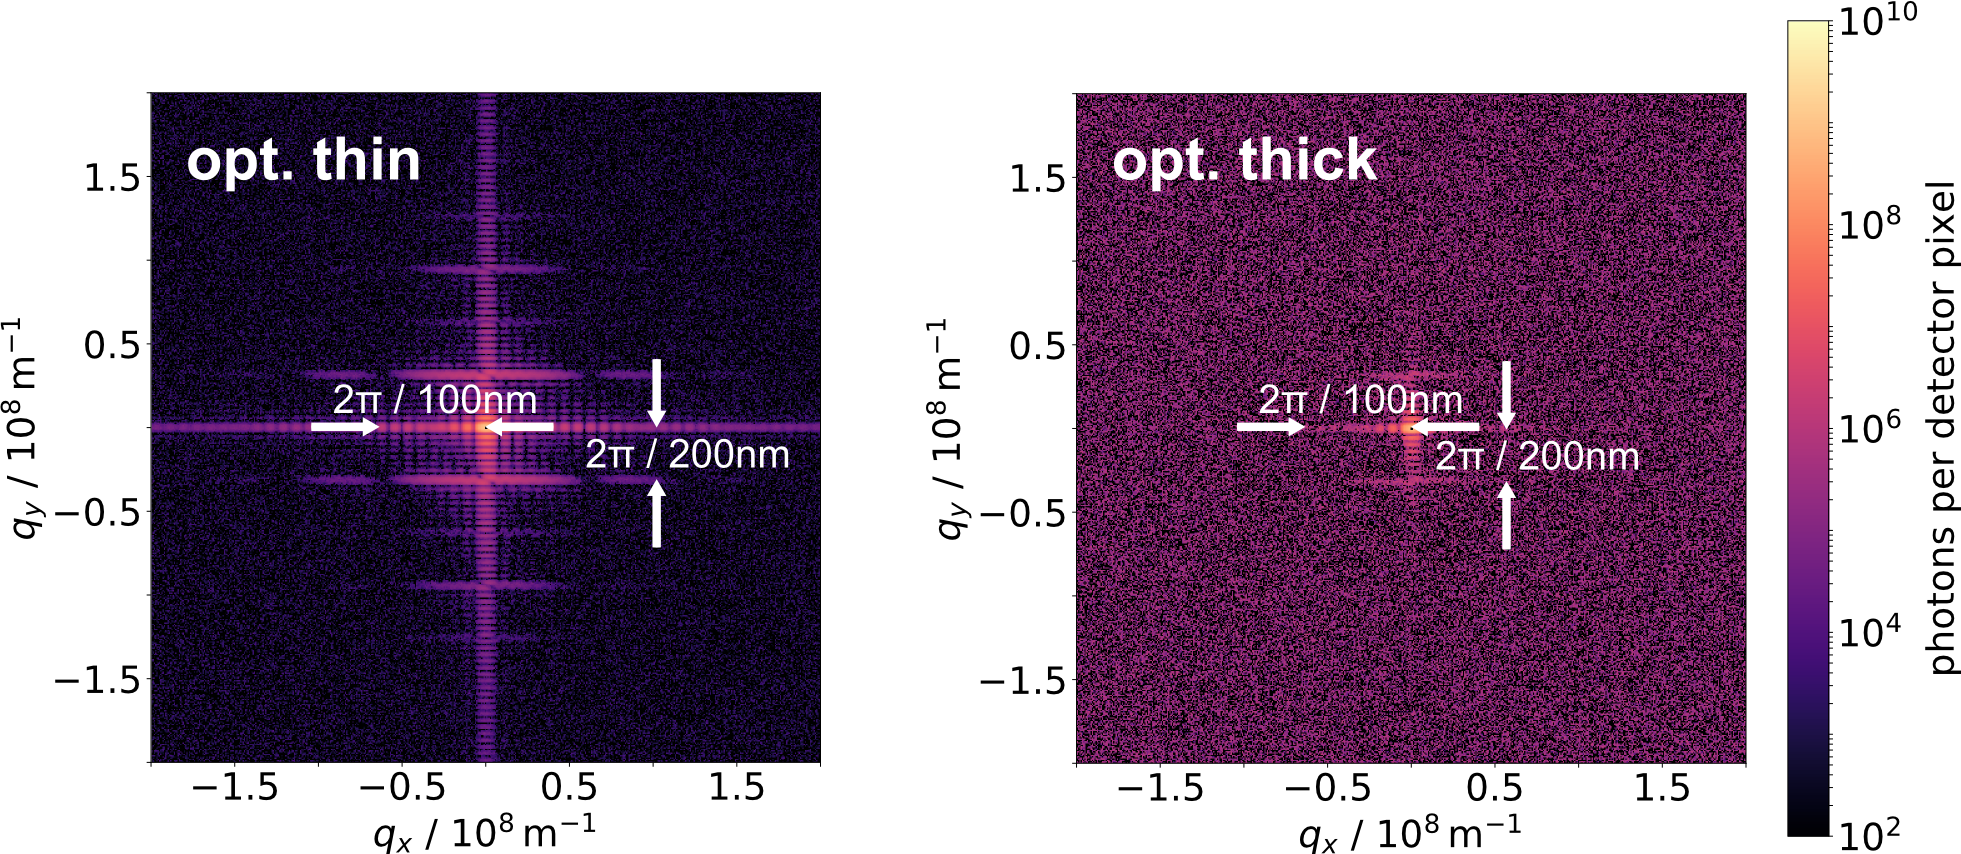
\includegraphics[width=.99\linewidth]{figures/scattering_images_v2.png}
  \caption{
    \textbf{Left:} \textit{ParaTAXIS} \gls{saxs} image for the optically thin target at
    $\SI{1.4}{\metre}$ distance from the target, detector pixel size $a_D =
    \SI{13.5}{\micro\metre}$, X-ray wavelength $\lambda_\mathrm{\gls{xfel}} =
    \SI{1.47}{\angstrom}$ and
    \num{e12} photons in the illuminated area. The vertical separation of scattering
    lines corresponds to the grating period of \SI{200}{\nano\metre}, the horizontal to
    the grating depth of \SI{100}{\nano\metre}.
    \textbf{Right:} \textit{ParaTAXIS} \gls{saxs} image for the optically thick target. Here, the
    scattering cross section was increased by a factor of \num{1000} to account for
  resonant scattering at the ion density. All other parameters remain the same.  }
  \label{fig:scattering}
\end{figure}

All density data from the \gls{pic} simulation as well as the \gls{saxs} patterns are
published on Zenodo together with the data format documentation
\cite{Garten2017.zenodo.885033} in partial fulfillment of EUCALL Milestone M4.4
\cite{EUCALL_SIMEX_M4.4}.

\section{Molecular (non--plasma) sample}
Application of \textit{simex\_platform} to single--particle imaging experiments
at the European X--ray Free Electron Laser (SPB--SFX scientific instrument) has
been published as Ref.~\cite{Fortmann-Grote2017}. It is also the basis for an
online tutorial on the
\href{https://www.github.com/eucall-software/simex_platform/wiki/SimEx-Tutorial}{wiki
pages} of \textit{simex\_platform} and it is
discussed in the EUCALL Milestone M4.2~\cite{EUCALL_SIMEX_M4.2} (First example
simulation).
The datasets for coherent diffraction from the protein 2NIP are deposited on
the \href{https://www.zenodo.org/communities/eucall-data}{EUCALL Data
Repository} \cite{Fortmann-Grote2017.zenodo.886087}.

The signal generation for non--plasma samples happens in two steps: First, the
photon--matter interaction module calculates for each time step of the
simulation the atomic positions and the atomic form factors for each
atom in the sample in the field of the x--ray laser. The effect of radiation
damage can be switched on or off in the simulation. In the latter case, the
atoms remain on their initial positions and the form factors correspond to the
atomic ground states.
This information is then
taken in the second step to calculate the scattered intensity as a function of
time for each pixel in the virtual 2D pixel detector. The software package
\textit{pysingfel} \cite{pysingfel_github} implements the scattering formula
\begin{equation}
  I(\mathbf{q}) = \Omega
  \frac{d\sigma_\mathrm{Th}(\theta)}{d\Omega}\langle I_0\rangle\left|
  \sum_i f_i(\mathbf{q})\mathrm{e}^{i\mathbf{q}\cdot\mathbf{R_i}}\right|^2~,
  \label{eqn:scattering_intensity}
\end{equation}
where $d\sigma_\mathrm{Th}/d\Omega$ is the differential Thomson cross
section,
$\langle I_0\rangle$ is the average pulse intensity, $\Omega$ is the solid
angle spanned by the considered detector pixel.
The wavevector $\mathbf{q}$ depends on the detector geometry (distance
$d$ from the sample) and pixel coordinates ($r_x, r_y$) in the detector plane assumed
to be perpendicular to the beam propagation axis and centered such that the
beam axis intersects the detector plane at its origin:
\begin{equation}
  q=\frac{2\pi}{\lambda}\left(%
  \begin{array}{l}
  \sin(2\theta)\,\cos(\phi)\\
  \sin(2\theta)\,\cos(\phi)\\
  \cos(2\theta)-1
  \end{array}%
  \right) =
  \frac{2\pi}{\lambda}\left(%
  \begin{array}{l}
    \frac{r_x}{\sqrt{r_x^2+r_y^2+d^2}}\\
    \frac{r_y}{\sqrt{r_x^2+r_y^2+d^2}}\\
    \frac{d-\sqrt{r_x^2+r_y^2+d^2}}{\sqrt{r_x^2+r_y^2+d^2}}
  \end{array}%
  \right)~.
  \label{eqn:q_components}
\end{equation}
%$q=\left|\mathbf{q}\right| = 4\pi/\lambda\,\sin(\theta)$.
Here, $2\theta=\arctan\left(\frac{r_x^2+r_y^2}{d}\right)$ is the scattering
angle and $\phi=\arctan\left(\frac{r_y}{r_x}\right)$. In this notation, the
pixel solid angle becomes
$\Omega=4\arcsin\left(a^2/\left[ 4(r_x^2+r_y^2+d^2)+a^2 \right]\right)$, with the pixel
width $a$.

In our simulations, $d=\SI{13}{\centi\metre}$. The
detector is a $512\times512$ array of pixels of side length
$a=\SI{200}{\micro\metre}$ corresponding to one quadrant of a 1 megapixel AGIPD
detector \cite{Allahgholi2015} at the SPB--SFX instrument at European XFEL.

We have applied this simulation toolchain to two cases:
\begin{enumerate}
  \item Diffraction of 5 keV photons from isolated 2NIP molecules and variation
    of the \gls{xfel} pulse duration, published in Ref.~\cite{Fortmann-Grote2017}.
  \item Diffraction of 5 keV photons from hydrated 2NIP molecules and variation
    of the hydration layer thickness, published in
    Ref.~\cite{Fortmann-Grote2017b}.
\end{enumerate}
Fig.~\ref{fig:2nip_diffraction_RD_vs_noRD} shows diffraction patterns from
2NIP with and without radiation damage taken into account in the simulation.
%
\begin{figure}[ht]
  \begin{center}
    \subfloat[no radiation damage]{%
    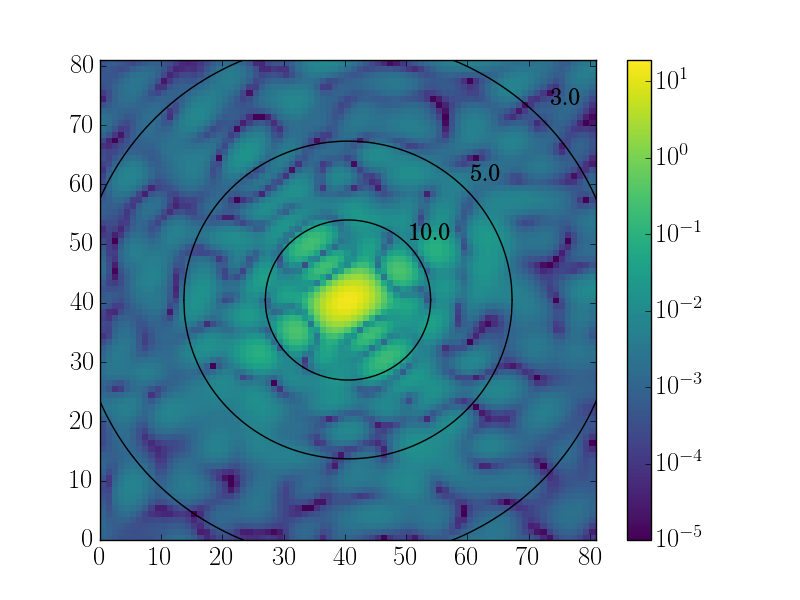
\includegraphics[width=0.4\textwidth,angle=0,clip]{figures/0000283_woRD}%
  }
    \subfloat[with radiation damage]{%
    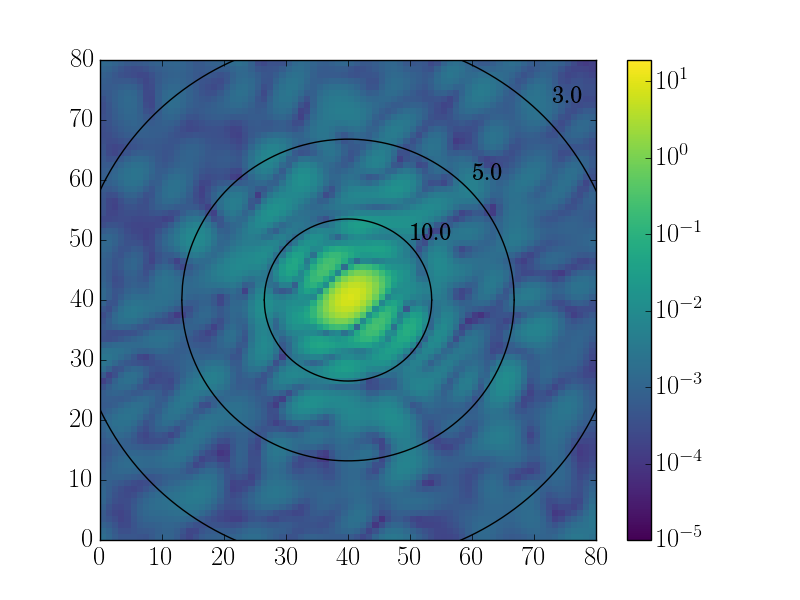
\includegraphics[width=0.4\textwidth,angle=0,clip]{figures/0000283_withRD}%
  }
  \end{center}
  \caption{Diffraction from 2NIP with 5 keV photons without (a) and with (b)
  radiation damage taken into account.}
  \label{fig:2nip_diffraction_RD_vs_noRD}
\end{figure}
%
Fig.~\ref{fig:2nip_hydration_layer} shows diffraction from the same molecule for
two different hydration layer thicknesses of \SI{3}{\angstrom} (a) and
\SI{10}{\angstrom} (b), respectively.
%
\begin{figure}[ht]
  \begin{center}
    \subfloat[\SI{3}{\angstrom} hydration layer]{%
    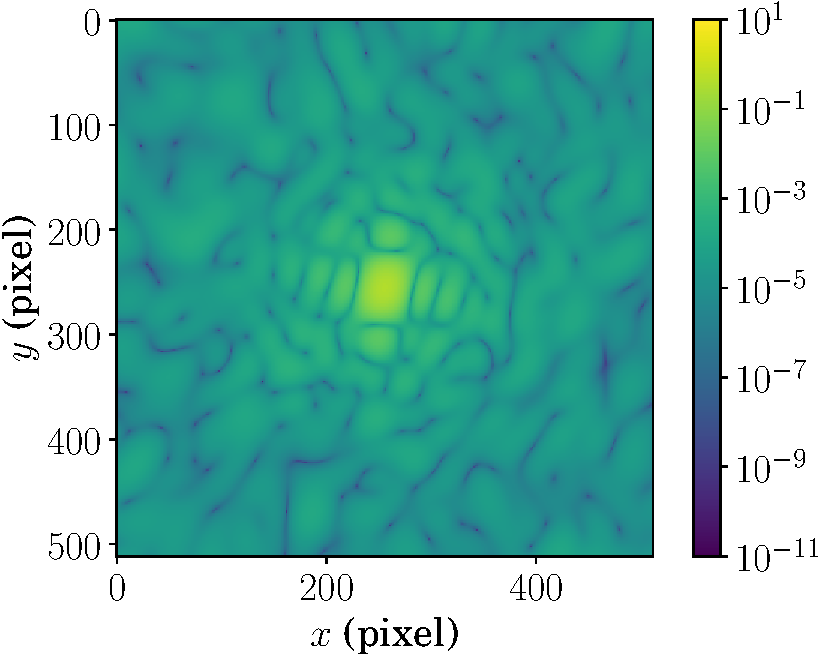
\includegraphics[width=0.4\textwidth,angle=0,clip]{2nip_1diffr_layer3-crop}
  }
    \subfloat[\SI{10}{\angstrom} hydration layer]{%
    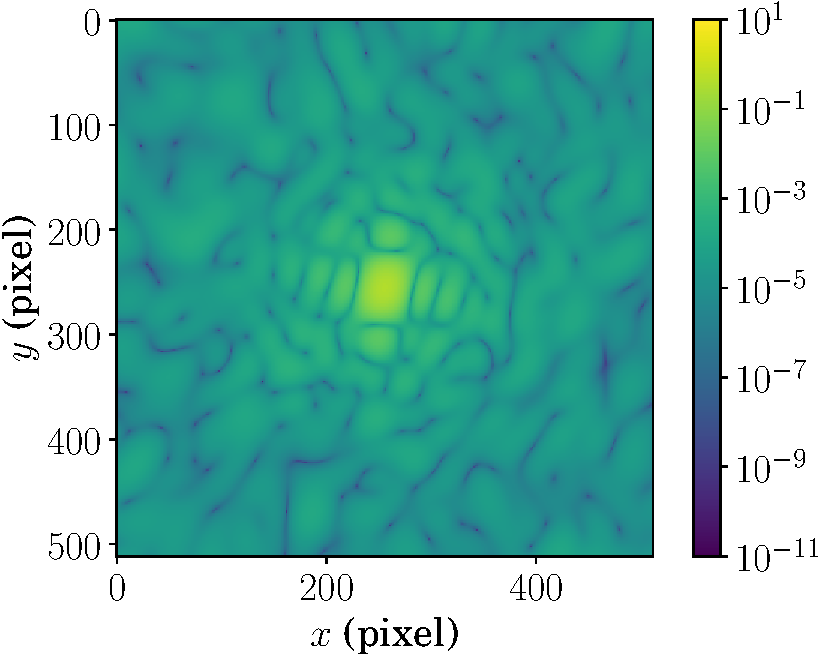
\includegraphics[width=0.4\textwidth,angle=0,clip]{2nip_1diffr_layer3-crop}
  }
  \end{center}
  \caption{Diffraction patterns for 5 keV XFEL photons scattering from a single
    2NIP molecule embedded in a hydration shell of \SI{3}{\angstrom} (a) and
    \SI{10}{\angstrom} (b) thickness.}
  \label{fig:2nip_hydration_layer}
\end{figure}

It can be seen how qualitatively, the presence of imperfections (radiation
damage and hydration layer) influences the quality of diffraction signals, e.g.
the speckle contrast and noise level.
In both cases, we performed statistical analysis of the simulated diffraction
patterns as a function of the varied parameters pulse duration and hydration
layer thickness, respectively to gain more quantitative insight into the
dependency of diffraction data quality on these effects. Results are published
in the aforementioned articles.

\printbibliography
%%%%%%%%%%%%%%%%%%%%%%%%%%%
\end{document}


